\documentclass{article}
\usepackage{graphicx} % Required for inserting images
\usepackage{listings}
\usepackage{tikz}
\newenvironment{cajarespuestas}{\begin{center}\fbox{\begin{minipage}{\linewidth}}}{\end{minipage}\end{center}}
\title{ICC Practica 03.1}
\author{Paolo Blanco Medina}
\date{October 2026}

\begin{document}

\maketitle
\section*{01 Referencias e inmutabilidad de String}
\subsection*{Código de la práctica}
\begin{lstlisting}[language=Java]
public class Ejercicio1 {
    public static void main(String[] args) {
        String a = "Java";
        String b = new String("Java");
        String c = "Ja" + "va";
        String d = "Ja";
        d += "va";
        System.out.println(a == b);
        System.out.println(a == c);
        System.out.println(a == d);
        System.out.println(a.equals(d));
        b = b.concat(" 21");
        System.out.println(a);
        System.out.println(b);
    }
}
\end{lstlisting}

\subsection*{Indica qué imprime cada instrucción y qué variables comparten un objeto.}
El programa imprime:
\begin{verbatim}
false
true
true
true
Java
Java 21
\end{verbatim}

\textbf{Análisis de cada instrucción:}
\begin{itemize}
    \item \textbf{System.out.println(a == b);} $\rightarrow$ \textbf{\texttt{false}}. Imprime false ya que evitamos el Pool al obligar a Java a crear un objeto en el heap con "new".
    \item \textbf{System.out.println(a == c);} $\rightarrow$ \textbf{\texttt{true}}. Imprime true ya que compara a ("Java") con c, este ultimo siendo "Ja" + "va" que es justamente igual a "Java".
    \item \textbf{System.out.println(a == d);} $\rightarrow$ \textbf{\texttt{false}}. Da false, ya que cuando se ejecuta la instrucción d += "va";, la concatenación involucra una variable en lugar de constantes puras, por lo que se resuelve en tiempo de ejecución. Java creó una nueva instancia en el Heap. Aunque el texto final resultante sea "Java", la dirección de memoria de d es distinta a la de a en el String Pool.
    \item \textbf{System.out.println(a.equals(d));} $\rightarrow$ \textbf{\texttt{true}}. El método \texttt{.equals()} evalúa la secuencia exacta de caracteres y no la dirección de memoria, por ende da true a diferencia de \textbf{Syste.out.println(a == d)}.
    \item \textbf{b = b.concat(" 21");} $\rightarrow$ Genera una nueva cadena \texttt{"Java 21"} en memoria que se asigna a la variable b, por eso \textbf{System.out.println(b)} imprime "Java 21".
    \item \textbf{System.out.println(a);} $\rightarrow$ \textbf{\texttt{Java}}. Solo imprime "Java"ya que es el valor de la variable, y esta no sufrió algun cambio
    \end{itemize}

\textbf{Variables que comparten objeto:} Las variables \textbf{\texttt{a}} y \textbf{\texttt{c}} comparten la misma referencia en el \textit{String Pool}.

\subsection*{Conceptos}
\begin{description}
    \item[String Pool:] Es una región especial dentro del Heap gestionada por la JVM para la optimización de memoria. Almacena una única copia de cada String, lo que evita duplicados cuando se crean cadenas idénticas.
    \item[Diferencia entre \texttt{==} y \texttt{equals()}:]
    \item \texttt{==}: Compara. 
    \item \texttt{equals()}: Compara el contenido o valor.
    \item[Comportamiento de \texttt{concat()}:] Crea y retorna una nueva instancia de String con el resultado de la concatenación.
\end{description}

\newpage

\section*{02 Operaciones e índices en StringBuilder}

\subsection*{Código de la práctica}
\begin{lstlisting}[language=Java]
StringBuilder sb = new StringBuilder("ABCDE");
sb.delete(1, 4);
sb.insert(1, "xyz");
sb.reverse();
sb.replace(1, 4, "-");
System.out.println(sb);
System.out.println(sb.length());
System.out.println(sb.capacity());
\end{lstlisting}

\subsection*{1. Salida y contenido}
\begin{enumerate}
    \item \texttt{sb = "ABCDE"}
    \item \textbf{sb.delete(1, 4):} Elimina los caracteres entre la posición 1 a la 4, quedando solo \texttt{"AE"}.
    \item \textbf{\texttt{sb.insert(1, "xyz"):}} Inserta la cadena \texttt{"xyz"} a partir de la posición del índice 1. Quedando \texttt{"AxyzE"}.
    \item \textbf{\texttt{sb.reverse():}} Invierte el orden de la secuencia completa de caracteres.\texttt{"Exyza"}.
    \item \textbf{\texttt{sb.replace(1, 4, "-"):}} Reemplaza los caracteres entre los índices 1  y 4, correspondientes a \texttt{"xyz"}, por el carácter \texttt{"-"}, siendo la salida \texttt{"E-a"}.
\end{enumerate}

\textbf{Salida exacta producida por los \texttt{System.out.println}:}
\begin{verbatim}
E-a
3
21
\end{verbatim}

\subsection*{2. Explicación de índices, \texttt{length()} y \texttt{capacity()}}
\begin{itemize}
    \item \textbf{¿Por qué \texttt{delete(1, 4)} no elimina cuatro caracteres?} \\
    En Java, la manipulación de rangos sobre secuencias se lee así [x, y). Por ende el 4 siempre queda excluido.
    \item \textbf{Diferencia entre \texttt{length()} y \texttt{capacity()}:}
    \begin{itemize}
        \item \texttt{length()}: Retorna la cantidad de caracteres.
        \item \texttt{capacity()}: Retorna el tamaño total de la memoria reservada internamente, la cual por defecto es la longitud inicial más 16 ($5 + 16 = 21$).
    \end{itemize}
\end{itemize}

\newpage

\section*{03 Referencias compartidas}

\subsection*{Código de la práctica}
\begin{lstlisting}[language=Java]
StringBuilder a = new StringBuilder("Hola");
StringBuilder b = a;
StringBuilder c = new StringBuilder("Hola");
a.append(" mundo");
b.delete(0, 5);
System.out.println(a);
System.out.println(b);
System.out.println(c);
System.out.println(a == b);
System.out.println(a.equals(b));
System.out.println(a.equals(c));
\end{lstlisting}

\subsection*{1. Salidas y explicación de modificaciones}
\textbf{Salida exacta:}
\begin{verbatim}
mundo
mundo
Hola
true
true
false
\end{verbatim}

\textbf{Análisis de modificaciones:}
\begin{itemize}
    \item \texttt{StringBuilder b = a;} asigna la referencia del objeto \texttt{a} a la variable \texttt{b}. Ambos identificadores apuntan al mismo espacio de memoria en el Heap.
    \item \texttt{a.append(" mundo");} modifica el objeto compartido, cambiando su contenido a \texttt{"Hola mundo"}.
    \item \texttt{b.delete(0, 5);} elimina los primeros 5 caracteres (\texttt{"Hola "}) sobre el mismo objeto referenciado por \texttt{b} y \texttt{a}, dejando el buffer con el valor \texttt{"mundo"}.
    \item \texttt{System.out.println(a);} e \texttt{println(b);} imprimen \textbf{\texttt{mundo}} dado que apuntan a la misma entidad.
    \item \texttt{System.out.println(c);} imprime \textbf{\texttt{Hola}}, ya que \texttt{c} se mantuvo como un objeto independiente en una dirección de memoria distinta.
    \item \texttt{System.out.println(a == b);} retorna \textbf{\texttt{true}} porque ambos almacenan exactamente la misma dirección de memoria.
    \item \texttt{System.out.println(a.equals(b));} retorna \textbf{\texttt{true}}.
    \item \texttt{System.out.println(a.equals(c));} retorna \textbf{\texttt{false}}. La clase \texttt{StringBuilder} \textbf{no sobreescribe} el método \texttt{equals()} de \texttt{java.lang.Object}. Por ende, \texttt{equals()} en \texttt{StringBuilder} realiza una comparación idéntica a \texttt{==} (por referencia) y no por contenido textual.
\end{itemize}

\subsection*{2. Esquema de memoria}

\begin{center}
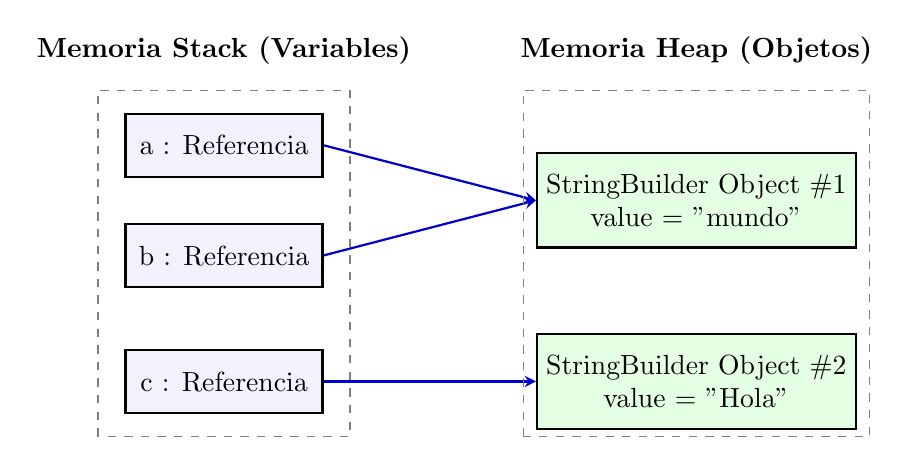
\begin{tikzpicture}[
    box/.style={rectangle, draw=black, fill=blue!5, thick, minimum width=2.5cm, minimum height=0.8cm, align=center},
    heapbox/.style={rectangle, draw=black, fill=green!10, thick, minimum width=3.5cm, minimum height=1.2cm, align=center},
    arrow/.style={->, >=stealth, thick, color=blue!80!black}
]

    % STACK
    \node[font=\bfseries] (stacklabel) at (0, 3.0) {Memoria Stack (Variables)};
    \node[box] (varA) at (0, 1.8) {a : Referencia};
    \node[box] (varB) at (0, 0.4) {b : Referencia};
    \node[box] (varC) at (0, -1.2) {c : Referencia};

    % HEAP
    \node[font=\bfseries] (heaplabel) at (6, 3.0) {Memoria Heap (Objetos)};
    \node[heapbox] (obj1) at (6, 1.1) {StringBuilder Object \#1\\value = "mundo"};
    \node[heapbox] (obj2) at (6, -1.2) {StringBuilder Object \#2\\value = "Hola"};

    % ARROWS
    \draw[arrow] (varA.east) -- (obj1.west);
    \draw[arrow] (varB.east) -- (obj1.west);
    \draw[arrow] (varC.east) -- (obj2.west);

    % DOTTED BOXES
    \draw[dashed, gray] (-1.6, -1.9) rectangle (1.6, 2.5);
    \draw[dashed, gray] (3.8, -1.9) rectangle (8.2, 2.5);

\end{tikzpicture}
\end{center}

\newpage

\section*{Preguntas apartado 10}

\begin{enumerate}
    \item \textbf{\bfseries ¿Por qué los atributos del editor deben ser privados?}
    
    \textbf{R:} Para hacer más robusto el código al encapsular las variables, y que otros métodos no cambien por error la memoria de la variable.

    \item \textbf{\bfseries ¿Qué diferencia hay entre un método public y uno private?}
    
    \textbf{R:} Lo accesible que son, Public puede ser alterado en cualquier parte del proyecto, mientras que private solo en la clase en la que está.

    \item \textbf{\bfseries Si quitas public de un método, ¿qué acceso tiene y puede llamarlo PruebaEditor desde el mismo paquete?}
    
    \textbf{R:} Si cambio public por private no tendrá acceso para PruebaEditor y no podrás llamarlo.

    \item \textbf{\bfseries ¿En qué se diferencia el acceso de paquete de protected?}
    
    \textbf{R:} El protected es igual que el private, pero añade un permite acceso a clases del mismo paquete y subclases (las cuales pueden estar en diferentes paquetes) por medio de la herencia.
\end{enumerate}

\end{document}
